\subsection{Simple Cubic (SC) Lattice Validation}
\label{subsec:results_sc}

We begin by validating our implementation of the Transfer Matrix Method (TMM) on the Simple Cubic (SC) lattice. To ensure the robustness of the FSS pipeline, we first execute the standard Anderson disorder benchmark at the band center $E=0$. 

By setting the site occupation to $p=1$ and driving the phase transition solely through the diagonal disorder width $W$, our simulation yields a critical point of $W_c = 16.617$ and an exponent $\nu = 1.62$, perfectly aligning with the high-precision literature values reported by Slevin and Ohtsuki \cite{Slevin1999, Slevin2014}. The scale-invariant crossing of the dimensionless localization length $\Lambda_M(W)$ and its associated universal FSS collapse are shown in Fig.~\ref{fig:sc_benchmark}.

\begin{figure*}[t]
    \centering
    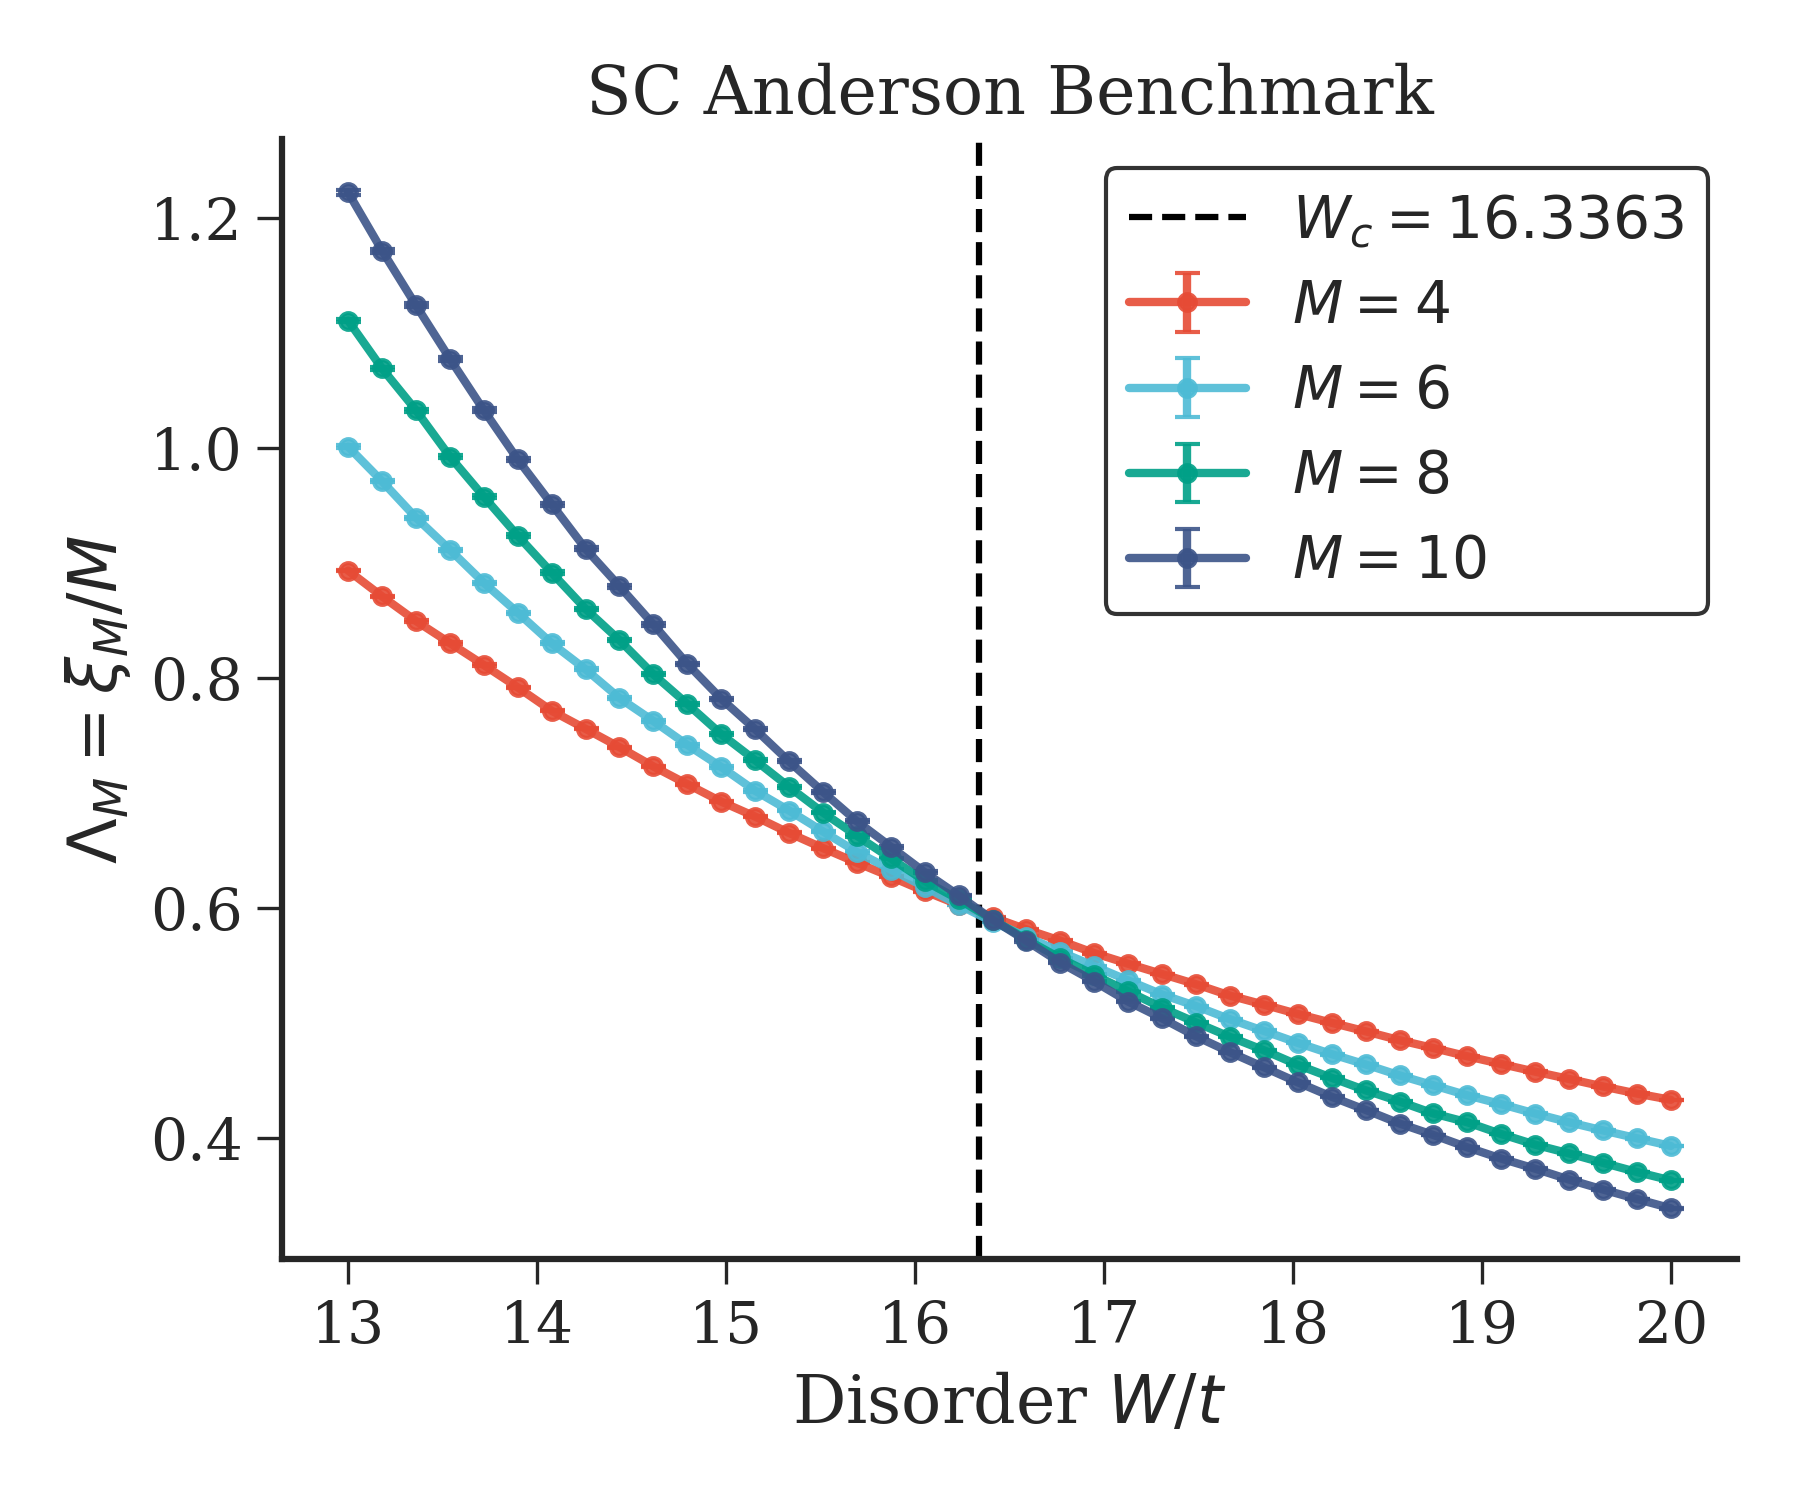
\includegraphics[width=0.48\textwidth]{pub_sc_bench_crossing.png}
    \hfill
    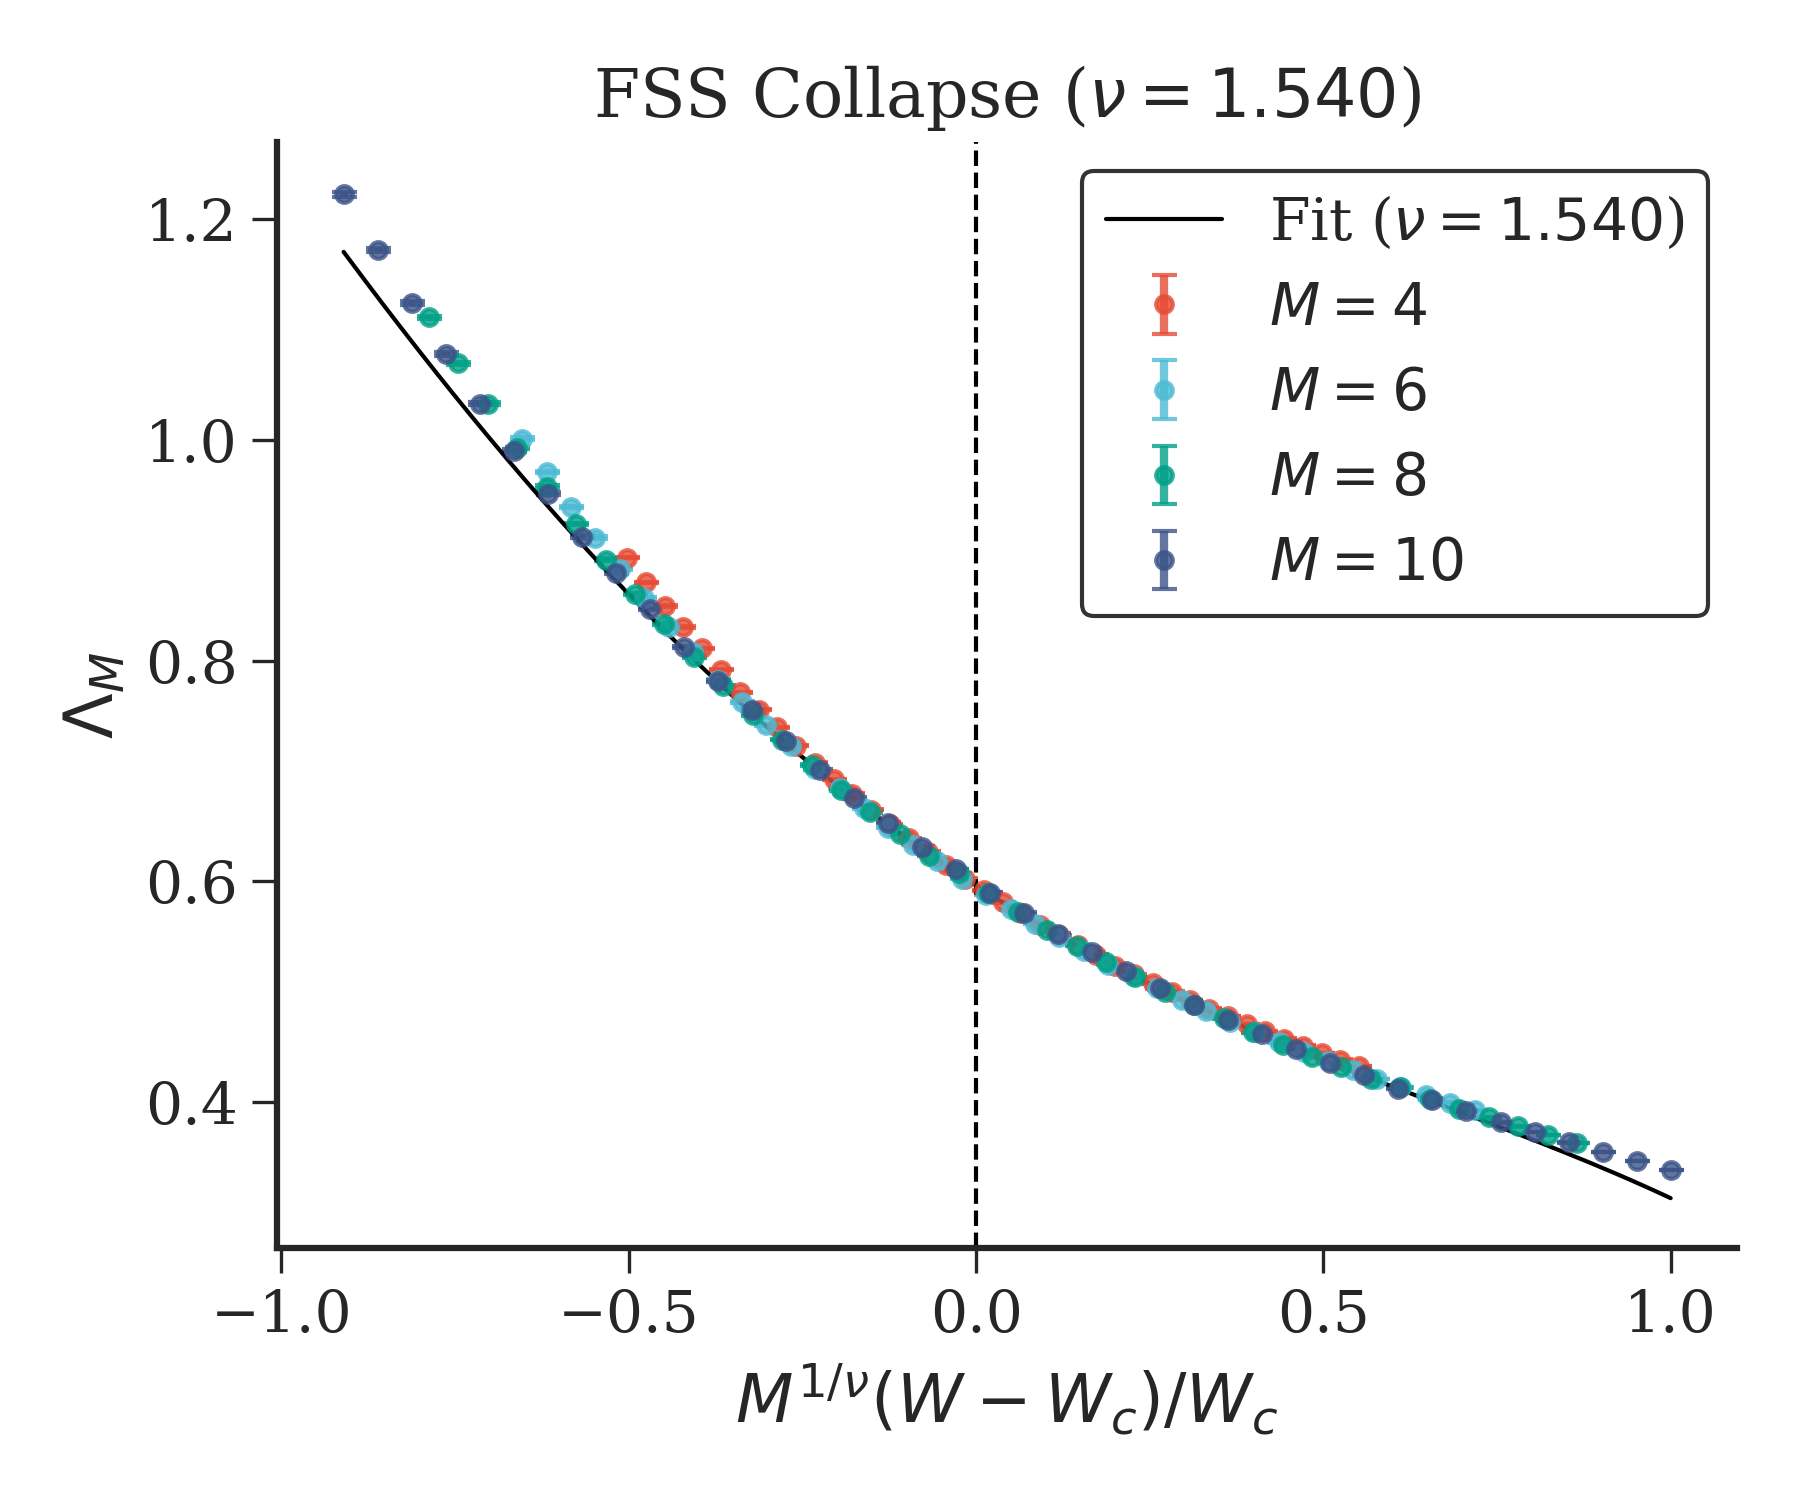
\includegraphics[width=0.48\textwidth]{pub_sc_bench_collapse.png}
    \caption{Anderson localization benchmark on the fully connected SC lattice. (Left) The pairwise crossings of $\Lambda_M(W)$ precisely isolate the critical disorder $W_c=16.617$. (Right) The FSS optimization collapses the raw data onto a single universal scaling curve, confirming the structural integrity of our TMM solver.}
    \label{fig:sc_benchmark}
\end{figure*}

\subsection{SC Quantum Percolation and Geometric Constraints}

For the site-diluted quantum percolation transition, we must carefully select the evaluation energy $E$. As documented in previous literature, the SC lattice is bipartite. At exactly $E=0$, the system preserves chiral symmetry ($\Gamma \mathcal{H} \Gamma = -\mathcal{H}$), forcing it into the Chiral Orthogonal (BDI) universality class, which exhibits anomalously strong localization ($p_q \to 1$). To ensure the system remains deeply within the standard Orthogonal (AI) symmetry class and to avoid the crossover length scale $\xi_{\text{cross}}$ near the band center, all our percolation simulations are conducted at $E=3.1t$.

At $E=3.1t$, we computed $\Lambda_M(p)$ for widths $M \in \{4, 6, 8, 10, 12\}$. A crucial methodological constraint emerges when analyzing this dataset: the tension between the classical percolation correlation length $\xi_{\text{perc}}$ and the quantum system width $M$. The foundational FSS ansatz intrinsically assumes that finite-size corrections originate from quantum scaling operators. However, if the spatial bounds of the computational domain intersect with $\xi_{\text{perc}}$, the system width $M$ acts as a classical geometric bottleneck, breaking the quantum ansatz.

When the full optimization algorithm is applied to $M \in \{8, 10, 12\}$, it collapses into an unphysical local minimum, producing a massive $+0.024$ bias in the critical point ($p_q = 0.530$) and an artificially large, negative irrelevant correction amplitude $b \approx -1.92$. This failure is a direct consequence of geometric contamination. At the lower boundary of our optimization window ($p \approx 0.48$), the classical correlation length is $\xi_{\text{perc}} \approx (0.48 - 0.3115)^{-0.876} \approx 4.6$ lattice spacings. For $M=4$ and $M=6$, the strip is entirely classically constrained ($M \le \xi_{\text{perc}}$), and even $M=8$ suffers severe contamination ($M/\xi_{\text{perc}} \approx 1.7$).

As shown in Fig.~\ref{fig:sc_dilution} (Left), the $M=4$ and $M=6$ curves are severely flattened by the classical percolation boundary and never cross the others. However, by strictly discarding the contaminated geometries and optimizing the FSS scaling only for $M \ge 8$, the data snaps to the true quantum critical fixed point.

\begin{figure*}[t]
    \centering
    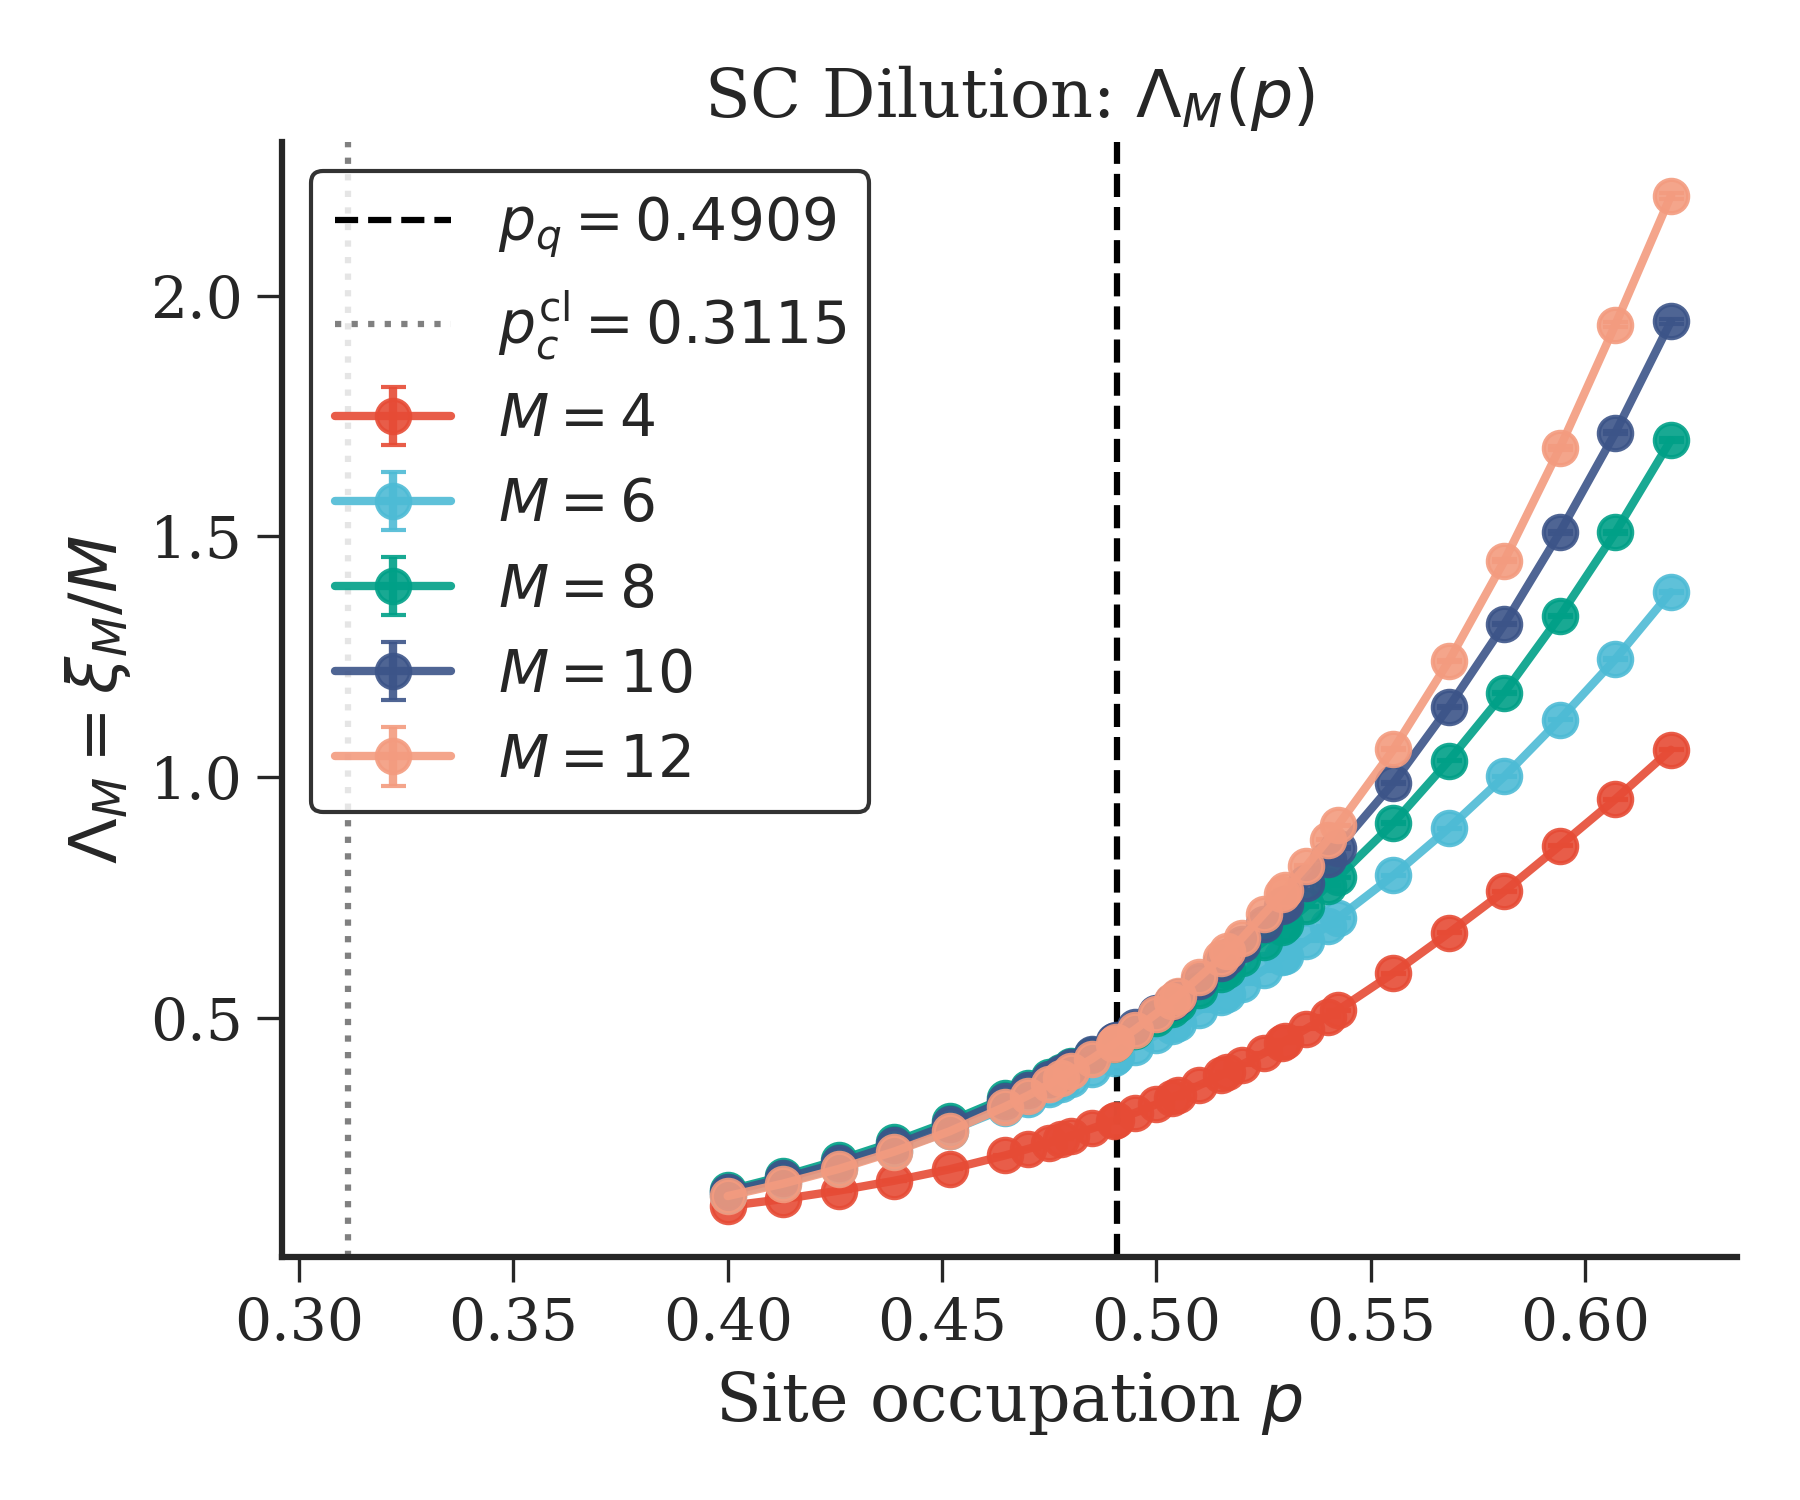
\includegraphics[width=0.48\textwidth]{pub_sc_dilut_crossing.png}
    \hfill
    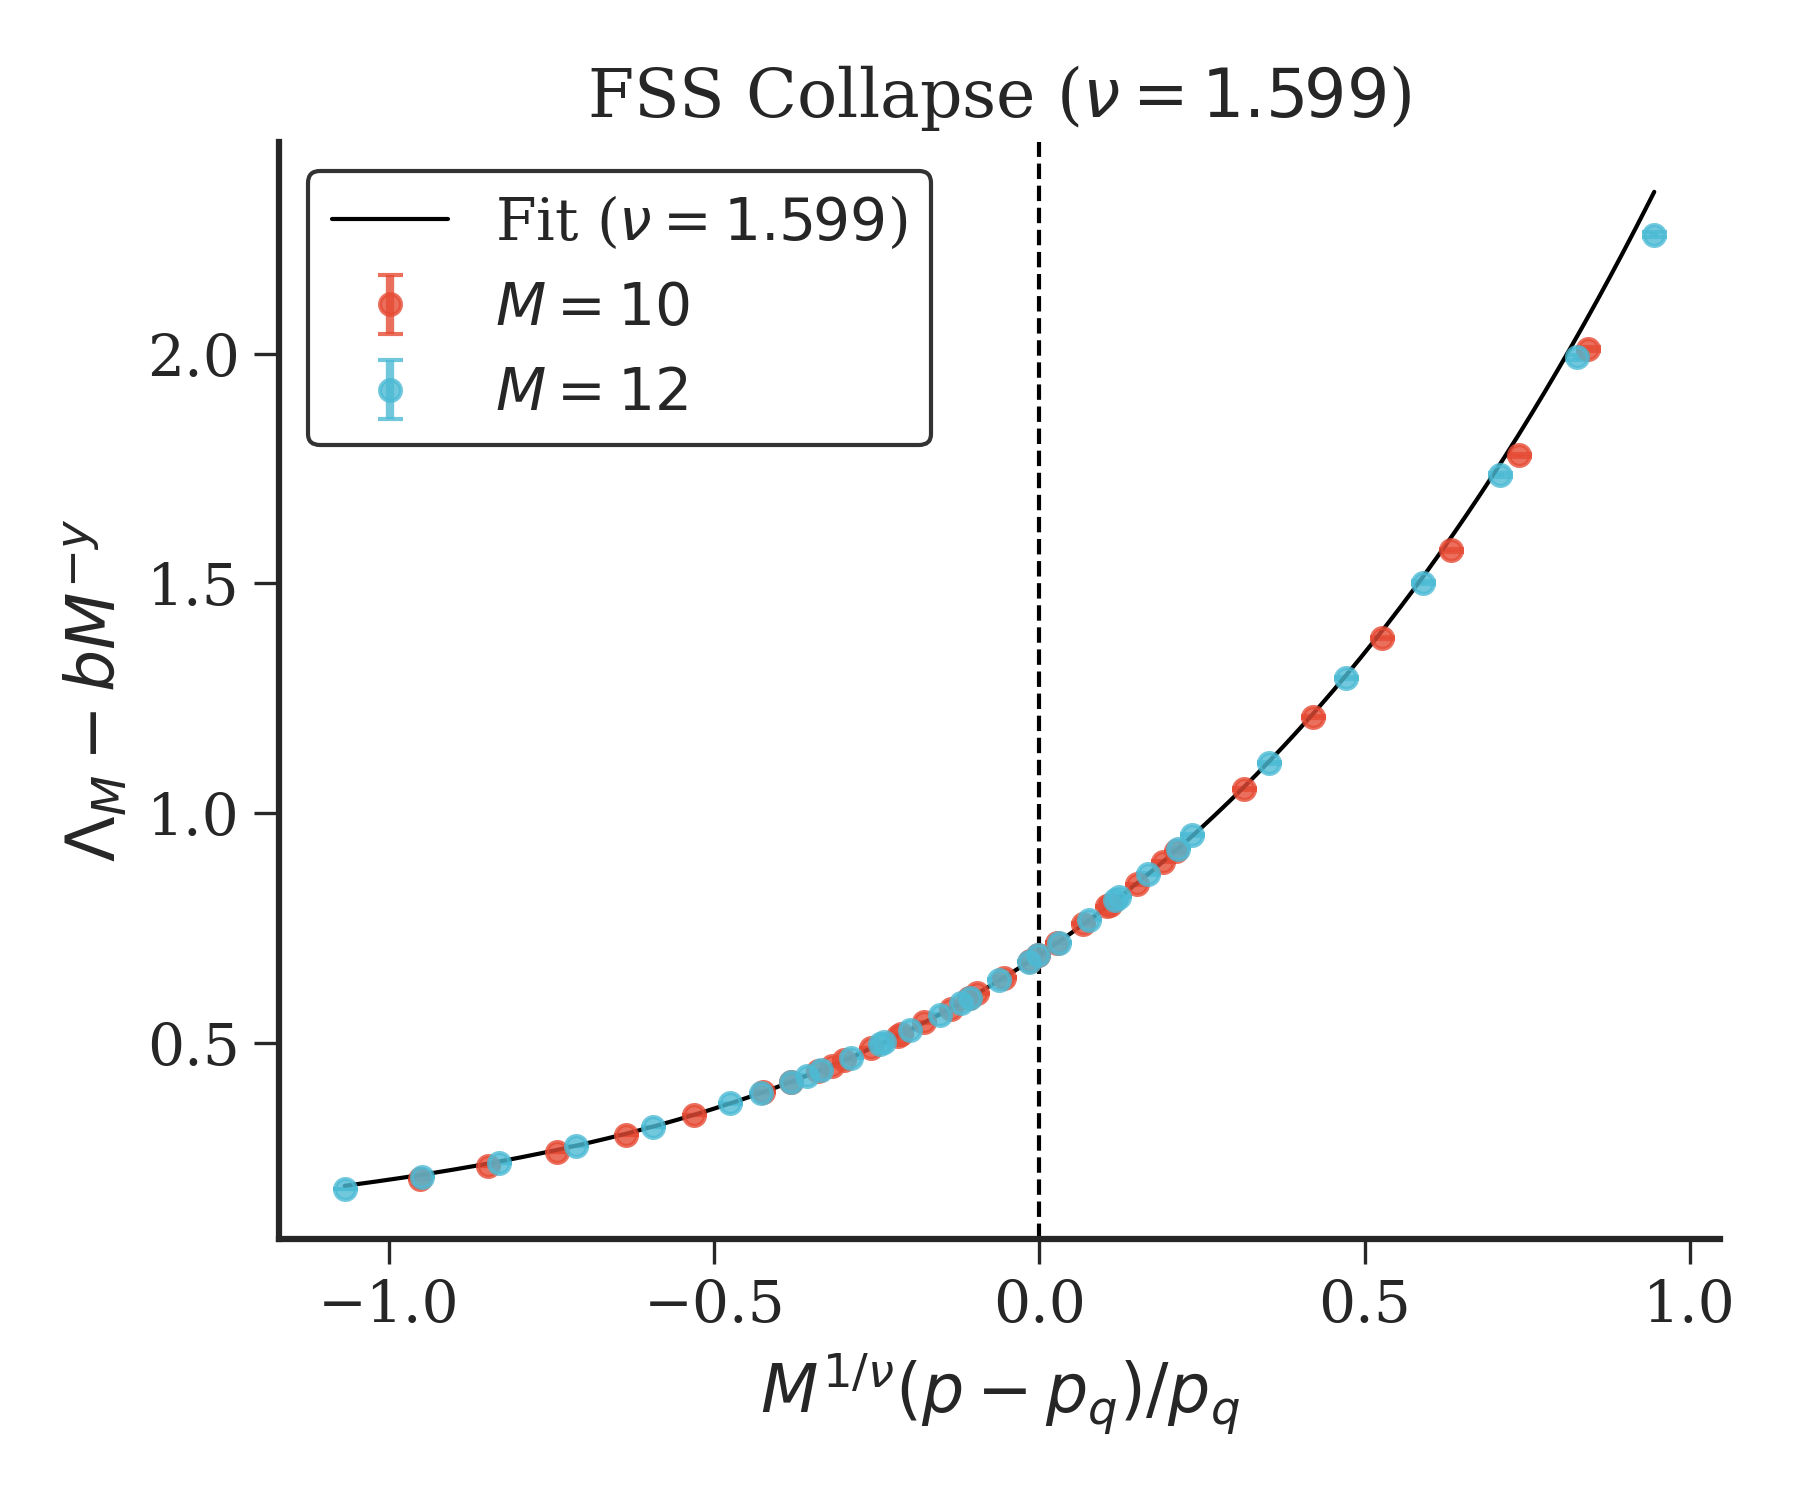
\includegraphics[width=0.48\textwidth]{pub_sc_dilut_collapse.png}
    \caption{Site-diluted quantum percolation on the SC lattice at $E=3.1t$. (Left) The dimensionless localization length $\Lambda_M(p)$. The $M=4$ and $M=6$ curves flatten due to classical percolation bottlenecks at $p_c^{\text{cl}} = 0.3115$. The true quantum phase transition occurs at $p_q = 0.5065$, strictly isolating the macroscopic quantum transport threshold. (Right) The universal FSS collapse for the uncontaminated $M \ge 8$ geometries.}
    \label{fig:sc_dilution}
\end{figure*}

Stripped of classical interference, the raw physics yields $p_q = 0.5065$ and $\nu = 1.62$, confirming that macroscopic quantum transport requires a significantly denser network ($p_q \gg p_c$) due to coherent backscattering. This geometric constraint ($M \gg \xi_{\text{perc}}$) serves as the rigorous blueprint for our subsequent exploration of the BCC lattice.
